\chapter{Aufgaben von Tag 3}

Die erste Aufgabe am dritten Tag besteht darin ein neuronales Netzwerk zu entwerfen, welches auf dem German Traffic Sign [...] 
korrekt klassifizieren kann. Im zweiten Aufgabenteil gilt es das neuronale Netzwerk zu einem konvolutinoalem Netzwerk auszubauen.
Um das Modell umzusetzen wird das Framework Tensorflow verwendet. Dieses Framework ist auf neuronale Netzwerke und Machine Learning 
Techniken spezialisiert. 

\subsection{Architektur des Netzwerkes}
Das Netzwerk besteht aus insgesamt vier vollständig verbundenen Schichten. Graphik \ref{img:nn_arch} skizziert die Architektur 
des Netzwerkes.
\begin{figure}
    \label{img:nn_arch}
    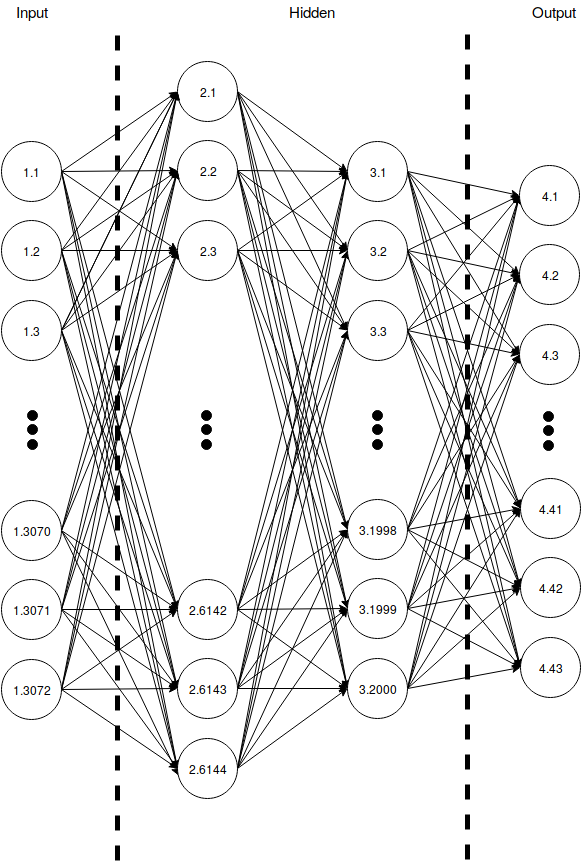
\includegraphics{Bilder/NeuralNetwork.png}
    \caption{Architektur des neuronalen Netzwerks}
\end{figure}
Jede der vier Schichten wird dargestellt, jedoch nicht jedes Neuron in der jeweiligen Schicht. Es werden jeweils die ersten drei 
und die letzten 3 Neuronen der Schicht angezeigt. Auf die Restlichen wurde der Übersichtlichkeit halber in der Graphik verzichtet.
Im dem mittels Tensorflow erstellten Graphen sind natürlich sämtliche Knoten vorhanden. 
In der ersten Schicht, der Input Schicht befinden sich 3072 Neuronen. Jedes Neuron nimmt einen Farbwert aus dem Bild auf. 
Diese gehen in die zweite Schicht über in welcher sich 6144 Neuronen befinden. Die dritte Schicht reduziert die Anzahl der Neuronen 
auf 2000 und leitet anschließend an die Output Schicht weiter, in welcher sich 43 Neuronen befinden. Jedes Output Neuron steht dabei 
für eine Verkehrsschild-Klasse. 

\subsection{Aufbereitung der Input-Daten}
Das Netzwerk erwartet einen Vektor als Eingabe. Dieser Vektor muss 3072 Elemente enthalten. Diese Anzahl ist sowohl durch die Höhe 
und Breite des Bildes gegeben, als auch durch die drei Farbmatrizen. Jede der drei Matrizen ist 32x32 Pixel groß. 
Der Datensatz, welcher für das Training genutzt wird, wird standardisiert um dessen Werte um 0 zu verteilen. 
Dazu wird die Formel: 
\begin{equation}
    x = \frac{\^{x} - mean}{\sigma}
\end{equation}
genutzt.

\subsection{Training}
Um das Netzwerk zu trainieren wird der Datensatz in einen Trainings-, eine Validierungs- und einen Test-Teil aufgesplittet. 
Die Lernrate ist auf 0.01 gesetzt und es werden insgesamt 40 Epochen trainiert. Zur Verbesserung des Netzwerkes wird das 
Gradientenverfahren angewandt. 